\documentclass[11pt,a4paper,x11names,twoside]{refart}

\usepackage{amsmath}
% Load multicolumn environment
\usepackage{multicol}
% Load tikz drawing environment
\usepackage{tikz}
% Load the additional options to load in pdf documents into the PDF
\usepackage{pdfpages}
% More control over the marginal notes environment.
\usepackage{marginnote}
% Colour
\usepackage[]{xcolor}
% Additional verbatim options
\usepackage{fancyvrb}
% Additional header/footer options
\usepackage{fancyhdr}
% Addition control over floats
\usepackage{float}
% Load in the last page marker.
\usepackage{lastpage}
% Addition bold mathematics options
\usepackage{bm}
% Load in the SI units options.
\usepackage[thinspace,thinqspace,squaren]{SIunits}
% Load in the tikz package for drawing circuit diagrams
\usepackage{circuitikz}
% Additional Font control for Lualatex and xelatex.
\usepackage{fontspec}
% Additional text symbols
\usepackage[full]{textcomp}

% Uncomment these if you want to use different fonts in the exam.
% Define the fonts for the exam. Namely Times New Roman as the main font, Helvetica as the sans serif font, and American Typewriter as the mono font. By default this will load the matching maths fonts
\setmainfont{TeX Gyre Termes}[Numbers=Lining,Ligatures={Common,Rare,TeX},Contextuals={WordInitial,Swash}]
\setsansfont{TeX Gyre Heros}[Numbers=Lining,Ligatures={Common,Rare,TeX},Contextuals={WordInitial,Swash}]
\setmonofont{Courier New}[Scale=MatchUppercase]


% Load additional tikz drawing libraries which are required for some exams.
\usetikzlibrary{positioning,arrows,calc,intersections}

% Define additional verbatim environments and commands.

\DefineVerbatimEnvironment{code}{Verbatim}%
{numbers=left,
  numbersep=3pt,
  frame=leftline,
  framesep=8pt,
  xleftmargin=10pt
}

\CustomVerbatimCommand{\codeinput}{VerbatimInput}%
{numbers=left,
  numbersep=3pt,
  frame=leftline,
  framesep=8pt,
  xleftmargin=10pt
}

\DefineVerbatimEnvironment{kbd}{Verbatim}%
{}



% Define the \examend command

\newcommand{\examend}[1]{~\vfill \maxipageruletrue\begin{maxipage}\centerline{\large \textbf{\textsc{End of Examination}}}\end{maxipage}\vfill}


% set the text fraction of the page
\settextfraction{0.8}

% Define the headers and footer for the exam. This will need to be modified for your exam as required.
\fancyhead[O]{\sffamily\textsc{\footnotesize Mat1100 — Foundation Mathematics  \hfill Page \thepage~of~\pageref{LastPage} \\
\hfill Examination Period — Semester 2, 2015\hfill }}
\fancyhead[E]{\sffamily\textsc{\footnotesize Page \thepage~of~\pageref{LastPage} \hfill Mat1100 — Foundation Mathematics  \\
\hfill Examination Period — Semester 2, 2015\hfill }}

\fancyfoot{}
\renewcommand{\headrulewidth}{0.5pt}
\renewcommand{\footrulewidth}{0.5pt}


% Define the Question and Marks environments
\newcommand{\qmarks}[1]{%
  #1~mark%
  \ifnum1=0#1\relax%
  \else%
  s%
\fi}
\newcommand{\question}[1]{\stepcounter{section}%
\section*{\sffamily{\textsc{Question~\arabic{section} \quad{\small{(\qmarks{#1})}}}}}}
%%%%%%%%%%%%%%%%
% Item with mark
\newcommand{\itemm}[1]{\item\mbox{$\!\!$}%
  \reversemarginpar\marginpar{\small\qmarks{#1}}}


  % Define a generic heading command
  \newcommand{\heading}[1]{\section*{\sffamily{\textsc{#1}}}}

  % Define the starting part (spart) and end part commands.
  \newcommand{\spart}[1]{ \maxipagerulefalse\begin{maxipage}\centerline{\sffamily\large \textbf{\textsc{Part #1}}}\end{maxipage}}
  \newcommand{\epart}[1]{ \maxipageruletrue\begin{maxipage}\centerline{\sffamily\large\textbf{\textsc{End of Part #1}}}\end{maxipage}}

% Define the label number levels her
  \def\theenumi{\alph{enumi}}
  \def\theenumii{\roman{enumii}}
  \def\theenumiii{\roman{enumiii}}
  \def\theenumiv{\arabic{enumiv}}
  \def\labelenumi{(\theenumi)}
  \def\labelenumii{(\theenumii)}
  \def\labelenumiii{(\theenumiii)}
  \def\labelenumiv{(\theenumiv)}

  % My exam custom commands
\renewcommand{\vec}[1]{\bm{#1}}
\newcommand{\ihat}{\widehat{\vec{i}}}
\newcommand{\jhat}{\widehat{\vec{j}}}
\newcommand{\khat}{\widehat{\vec{k}}}
\newcommand{\ds}{\displaystyle}
\newcommand{\script}{\textsc{Sci}/\textsc{Matlab}}
  \begin{document}
  % Included the front piece
  \pagenumbering{roman}
  %\newgeometry{margin=25mm}
  \includepdf[pages={1-2}]{front.pdf}
  \pagestyle{empty}

  % Set up the exam layout
  \pagestyle{fancy}
  \addtolength{\headheight}{\baselineskip}
  \fancyheadoffset[L]{3.2cm}
  \fancyfootoffset[L]{3.2cm}
  \setcounter{page}{1}
  \pagenumbering{arabic}


  \spart{A1}

  \begin{maxipage}
    \begin{center}
  Part A contains XX questions. Not all questions are worth the same marks. \\
  200 marks\\
  Please answer all questions.
\end{center}
\end{maxipage}
  \epart{A1}

  Åå ¬Ò˚ò$∂$≠$±$+–±—‚·°

  \spart{B}
  \epart{B}

  \heading{Special instructions}

  \begin{itemize}
    \item Answer all questions in the booklets provided.
    \item Show all working.
    \item Questions are not of equal value.
  \end{itemize}


  \question{14}
  \begin{enumerate}
    \itemm{3} Factorise:
      \[ 3s^2-s-2\;.\]
    \itemm{3} Solve the quadratic equation:
      \[ 3t^2-t-2=0\;.\]
    \itemm{4} Solve the following set of simultaneous equations for $a$ and $b$.
      \begin{eqnarray*}
        12a-18b &=& 20 \\
        a+2b &=& 5
      \end{eqnarray*}
    \itemm{4} Simplify the following:
      \[ \frac{(36x^6y^{12})^\frac{1}{2}}{3(x^{10}y^{15})^\frac{1}{5}}\;.\]

  \end{enumerate}
  \vfil
  \question{5} %M1 Theory Q13
If the Mean of a distribution is smaller than its Median the distribution of this sample is:
\begin{enumerate}
  \item	skewed left  % %answer
  \item	skewed right
  \item	is unlikely to have any outliers
  \item	symmetric
\end{enumerate}

  \question{1}

  \begin{enumerate}
    \itemm{1} Find the equation, and identify the slope and $y$-intercept for a
      straight line passing through the points $(-30, 25)$ and $(20,-30)$.
    \itemm{2}  Sketch the graph of: \[y = \frac{2}{(x -5)} +\frac{5}{2},\] showing the
      asymptotes and all intercepts.
    \itemm{4}  Determine the radius and centre of the circle:
      \[ x^2 +y^2 -8x+10y+31=0\;.\]

  \end{enumerate}
  \vfill

  \newpage
  \question{16}

  \begin{enumerate}
    \itemm{3} Simplify $\log(10^{2x})$.
    \itemm{3} Solve the following equation:
      \[ 8^{2x+1}=4096\;.\]
    \item USQ's Toowoomba campus has approximately $3000$ students, a single student  returns to campus after the break with the flu. The spread of flu through the  student population can be modelling by:
      \[ N(t)=\frac{3000}{1+2999e^{-0.8t}} \]
      where $N(t)$ is the number of Students with the flu $t$ days after the student returned.
      \begin{enumerate}
        \itemm{3} What value does $N$ have after $5$~days?
        \itemm{4} Find the value of $t$ when exactly half the students have the flu.
        \itemm{3}  Sketch a graph, choosing suitable scales on both axes, which shows how the number of students with the flu varied
          over $30$~days. (A sketch which shows the shape of the graph and its important properties, is fine.)

      \end{enumerate}

  \end{enumerate}

  \vfil
  \question{9}

  In the following question
  \[
    \mathbf{A}=\begin{bmatrix}4 & 8 \\ 9 & 10 \end{bmatrix}, \hspace{0.5cm}
    \mathbf{ B}=\begin{bmatrix}1 & 0  \\ 0 & 1  \end{bmatrix}, \hspace{0.5cm}
    \mathbf{ C}=\begin{bmatrix}6 & 8 & 6 \\ 0 & 9  & 7 \end{bmatrix}
  \]

  Find or state why it is not possible:
  \begin{enumerate}
    \itemm{3} $\mathbf{ A}\mathbf{ B}$


    \itemm{3} $\mathbf{A}^{-1}$


    \itemm{3} $\mathbf{A}\mathbf{C}$
  \end{enumerate}
  \newpage

  \question{16}
  \begin{enumerate}
    \itemm{3} Find all angles $\left(\rho\right)$ between $0$ and $2\pi$
      which satisfy the equation: \\
      \[\sin \rho = \frac{1}{\sqrt{2}}\;.\]
    \itemm{4} $ABC$ is a triangle in which $AB=\unit{100}{\milli\metre}$,
      $BC=\unit{150}{\milli\metre}$, and $\angle ABC=\unit{60}{\degree}$.
      Find length of $AC$. (\textsc{Diagram not to scale.})% \begin{figure}[h]
        \begin{center}
          \begin{tikzpicture}
            \draw (0,0) --  (5,0);
            \draw (-2,-3) -- (0,0);
            \draw (-2,-3) -- (5,0);
            \draw (0,0) node[above] {$B$};
            \draw (5,0) node[above] {$A$};
            \draw (-2,-3) node[below] {$C$};
            \draw (-1,-1.2) node[left] {$a=\unit{150}{\milli\metre}$};
            \draw (2.5,0) node[above] {$c=\unit{100}{\milli\metre}$};
            \draw (+0.,0) node[below right] {\unit{60}{\degree}};
          \end{tikzpicture}
        \end{center}

      \item A \unit{45}{\metre} lighthouse $(LC)$ is situated on the edge of a vertical ocean cliff, as shown on the diagram below (\textsc{not to scale}). Measurements from a ship offshore show, the angle of elevation of the top of the lighthouse is \unit{45}{\degree} (i.e. $\angle LSB$),  while the elevation of the base of the lighthouse is \unit{30}{\degree} (i.e. $\angle CSB$). Let the length $CB$ be $h$.

        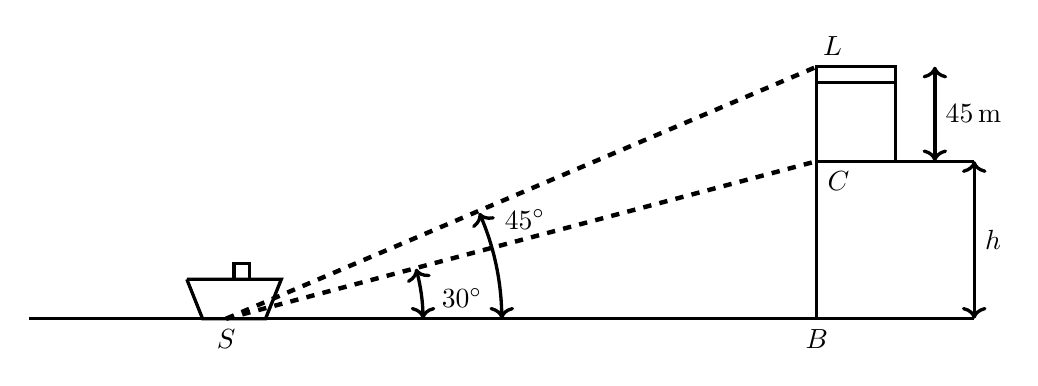
\begin{tikzpicture}[very thick]
          \draw (0,0) -- (12,0);
          \draw (10,0) -- (10,2) -- (12,2);
          \draw (10,2) -- (10,3) -- (11,3)-- (11,2);
          \draw (10,3) -- (10,3.2) -- (11,3.2) -- (11,3);1
          \draw (2,0.5) -- (2.2,0)  -- (3,0) -- (3.2,0.5) -- (2,0.5);
          \draw (2.6,0.5) -- (2.6,0.7) -- (2.8,0.7) -- (2.8,0.5);
          \draw[ultra thick,dashed] (2.5,0) -- (10,2);
          \draw[ultra thick,dashed] (2.5,0) -- (10,3.2);
          \node at (2.5,0) [below]  {$S$};
          \node at (10,0) [below] {$B$};
          \node at (10.2,3.2) [above] {$L$};
          \node at (10,2) [below right] {$C$};
          \draw[<->] (12,0) -- (12,2) node [midway,right] {$h$};
          \draw[<->] (11.5,2) -- (11.5,3.2) node [midway,right] {\unit{45}{\metre}};
          \draw[<->] (5,0) arc (0:16:2.3);
          \draw[<->] (6,0) arc (0:24:3.3);
          \node at (5.1,0) [above right] {\unit{30}{\degree}};
          \node at (5.9,1.0) [above right] {\unit{45}{\degree}};




        \end{tikzpicture}

        Using these measurements find the following:

        \begin{enumerate}
          \itemm{3}  The length of $SB$ in terms of $h$.
          \itemm{3} The length of $SB$  in terms of the length of $LB$.
          \itemm{3} Hence, or otherwise find the height of the cliff (i.e. length of $CB$).
        \end{enumerate}

    \end{enumerate}

    \newpage
    \vfil

    \question{16}
    Consider the vectors $\bm{a}=\ihat+3\jhat+2\khat$ and
    $\bm{b}=-2\ihat+4\jhat-\khat$. Find the following.
    \begin{enumerate}
      \itemm{2} $|\bm{a}|$
      \itemm{2} $|\bm{b}|$
      \itemm{4} The unit vector $\widehat{\bm{a}}$.
      \itemm{4} $\bm{a}\cdot\bm{b}$
      \itemm{4} The angle between $\bm{a}$ and $\bm{b}$.

    \end{enumerate}
    \question{17}


    \begin{enumerate}
      \item Differentiate with respect to $x$
        \begin{enumerate}
          \itemm{4} $5x^4+2x^2+x+10$
          \itemm{4} $5\sin{(\pi x)}$
        \end{enumerate}
      \item
        In a book the pages have an area of \unit{338}{\centi\metre\squared}. Each page has a left/right margin of \unit{1}{\centi\metre} and top/bottom margin of \unit{2}{\centi\metre} as shown in the diagram below (\textsc{not to scale}). If the page width is {$x$}~{\centi\metre} the printable area ($A$) shaded in the diagram is given by:
        \[ A(x)=346-4x-\frac{676}{x}.\]
        \begin{center}
          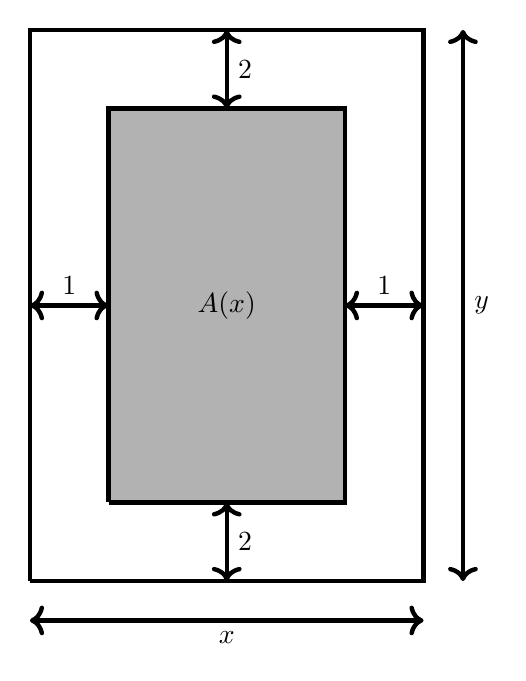
\begin{tikzpicture}[ultra thick]
            \draw (0,0) -- (5,0) -- (5,7) -- (0,7) -- (0,0);
            \draw[fill=black!30] (1,1) -- (4,1) -- (4,6) -- (1,6) -- (1,1);
            \node at (2.5,3.5) {$A(x)$};
            \draw[<->] (0,3.5) -- (1,3.5) node [midway,above] {$1$};
            \draw[<->] (4,3.5) -- (5,3.5) node [midway,above] {$1$};
            \draw[<->] (2.5,0) -- (2.5,1) node [midway,right] {$2$};
            \draw[<->] (2.5,6) -- (2.5,7) node [midway,right] {$2$};
            \draw[<->] (0,-0.5) -- (5,-0.5) node [midway,below] {$x$};
            \draw[<->] (5.5,0) -- (5.5,7) node [midway,right] {$y$};
          \end{tikzpicture}

        \end{center}

        \begin{enumerate}
          \itemm{4} Find $\ds\frac{dA}{dx}$.
          \itemm{5} Using your result in part b(i), find the dimensions of the page $(x,y)$ so that the printable area ($A$) is maximised.
        \end{enumerate}
    \end{enumerate}


    \newpage
    \newpage
    \appendix
    \section*{Table}

    \examend


    \end{document}
